% http://www.idt.mdh.se/phd/thesis/kthesis-1.0/
\documentclass[a4paper,11pt]{kthesis}
\usepackage[T1]{fontenc}
\usepackage[normalem]{ulem}
\usepackage[english]{babel}
\usepackage{listings,babel}
\lstset{breaklines=true,basicstyle=\ttfamily}
\usepackage{graphicx}
\usepackage{moreverb}
\usepackage{float}
\usepackage{cite}

\title{A performance-driven SoC architecture for video synthesis}
\date{June 2010}
\type{Master of Science Thesis in System-on-Chip Design}
\department{Department of Software and Computer Systems}
\author{S\'ebastien Bourdeauducq}
\imprint{Stockholm 2010}
\publisher{KTH}
\tmnotice{Milkymist is a trademark of S\'ebastien Bourdeauducq.}
\trita{xxx-nnnn}
\issn{nnnn-nnnn}
\isrn{KTH/xxx/R-{}-nn/n-{}-SE}
\isbn{x-xxxx-xxx-x}
\begin{document}
\begin{abstract}
TODO
\end{abstract}

\tableofcontents
\listoffigures

\mainmatter

\chapter{Introduction}
The open source model means that any individual, if he or she has the required level of technical knowledge, can realistically use, share and modify the design of a technical system. During the nineties, this development model gained popularity in the software world with, most notably, the GNU/Linux operating system. But it was not viable for complex SoCs until a few years ago, because the cost of prototyping semiconductor chips is prohibitive  and field programmable gate arrays (FPGA) used to be too slow, too small, and too expensive. System-on-chip design and hands-on computer architecture therefore remained a field reserved to well-funded academia and research and development laboratories of companies of a significant size and wealth, who had access to large FPGA clusters or even semiconductor foundries.

\begin{figure}[htp]
\centering
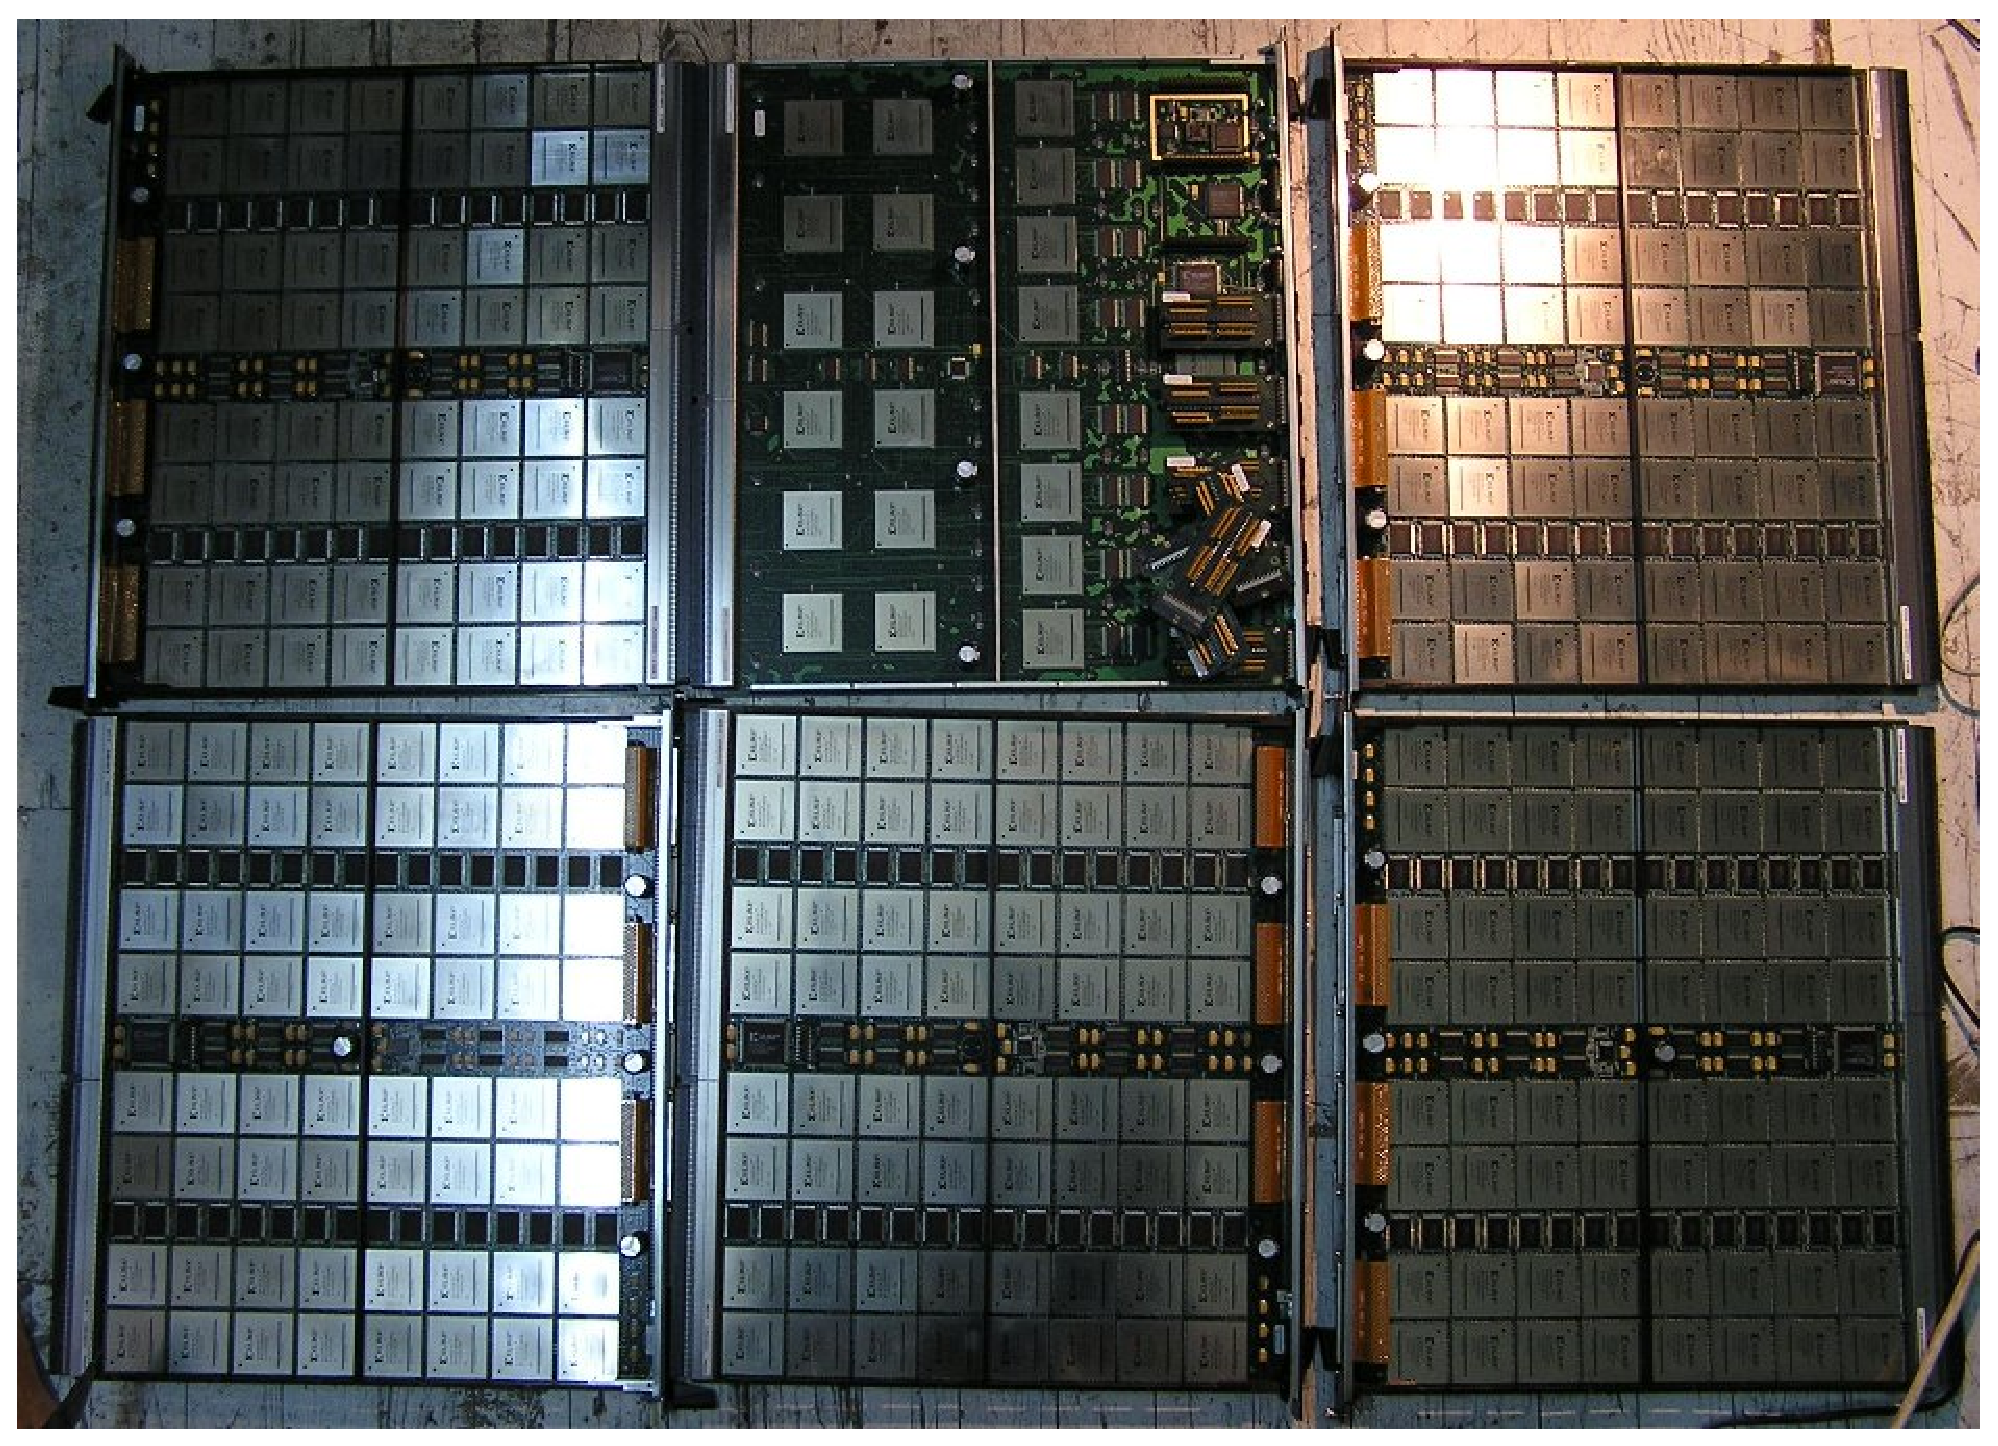
\includegraphics[height=95mm]{ikosboards.eps}
\caption{FPGA boards of the Ikos Pegasus ASIC emulator (ca. 1999)}
\label{fig:ikos}
\end{figure}

But today, the cost of fast high-density FPGAs is falling and these devices are becoming available to the general public. For an example of this trend, I would mention the Ikos Pegasus application specific integrated circuit (ASIC) emulator, whose insides are depicted in Figure~\ref{fig:ikos}. The CPU core used in the system-on-chip described in this thesis occupies alone 60\% of the resources of one of the XC4036XL FPGAs of this device, and runs at 30MHz. The Ikos Pegasus was a state-of-the-art device a decade ago. It consumes up to 3 kilowatts of power, weights dozens of kilos and costed the equivalent of several millions of SEK. The same CPU core now occupies about 15\% of a modern FPGA costing less than 500 SEK, where it runs in excess of 100MHz.

This evolution makes it possible to implement complex high-performance system-on-chips (SoC) that can be modified and improved by anyone, thanks to the flexibility of the FPGA platform.

This master thesis introduces Milkymist\texttrademark \cite{Milkymist}, a fast and resource-efficient FPGA-based system-on-chip designed for the application of rendering live video effects during performances such as concerts, clubs or contemporary art installations. Such effects are already popularized by artists known as ``video jockeys'', or ``VJs''.

Besides the fact that this is an interesting, creative and popular application, it is also demanding in terms of computational power and memory performance. It would make Milkymist a proof that high performance open source system-on-chip design is possible in practice; with a view to help, foster and catalyze similar ``open hardware'' initiatives. As the Milkymist system-on-chip is entirely made of synthesizable Verilog and, for the most part, released under the GNU GPL, its code can be re-used by other open hardware projects.

Meeting the performance constraints while still using cheap and relatively small FPGAs is perhaps the most interesting and challenging technical point of this project, and it could not be done without considerable work in the field of computer architecture. This is what this master thesis covers.

\section{Background}
\subsection{Video synthesis}
MilkDrop~\cite{milkdrop} is a popular open source video synthesis framework that was originally made to develop visualization plugins for the Winamp audio player. People have since then ported MilkDrop to many different platforms and made it react to live events, such as captured audio or movements of a WiiMote remote control.

The idea behind the Milkymist project is to implement an embedded video synthesis platform on a custom open source system-on-chip that is based on the same rendering principle of MilkDrop, but with more control interfaces and features.

\begin{figure}[htp]
\centering
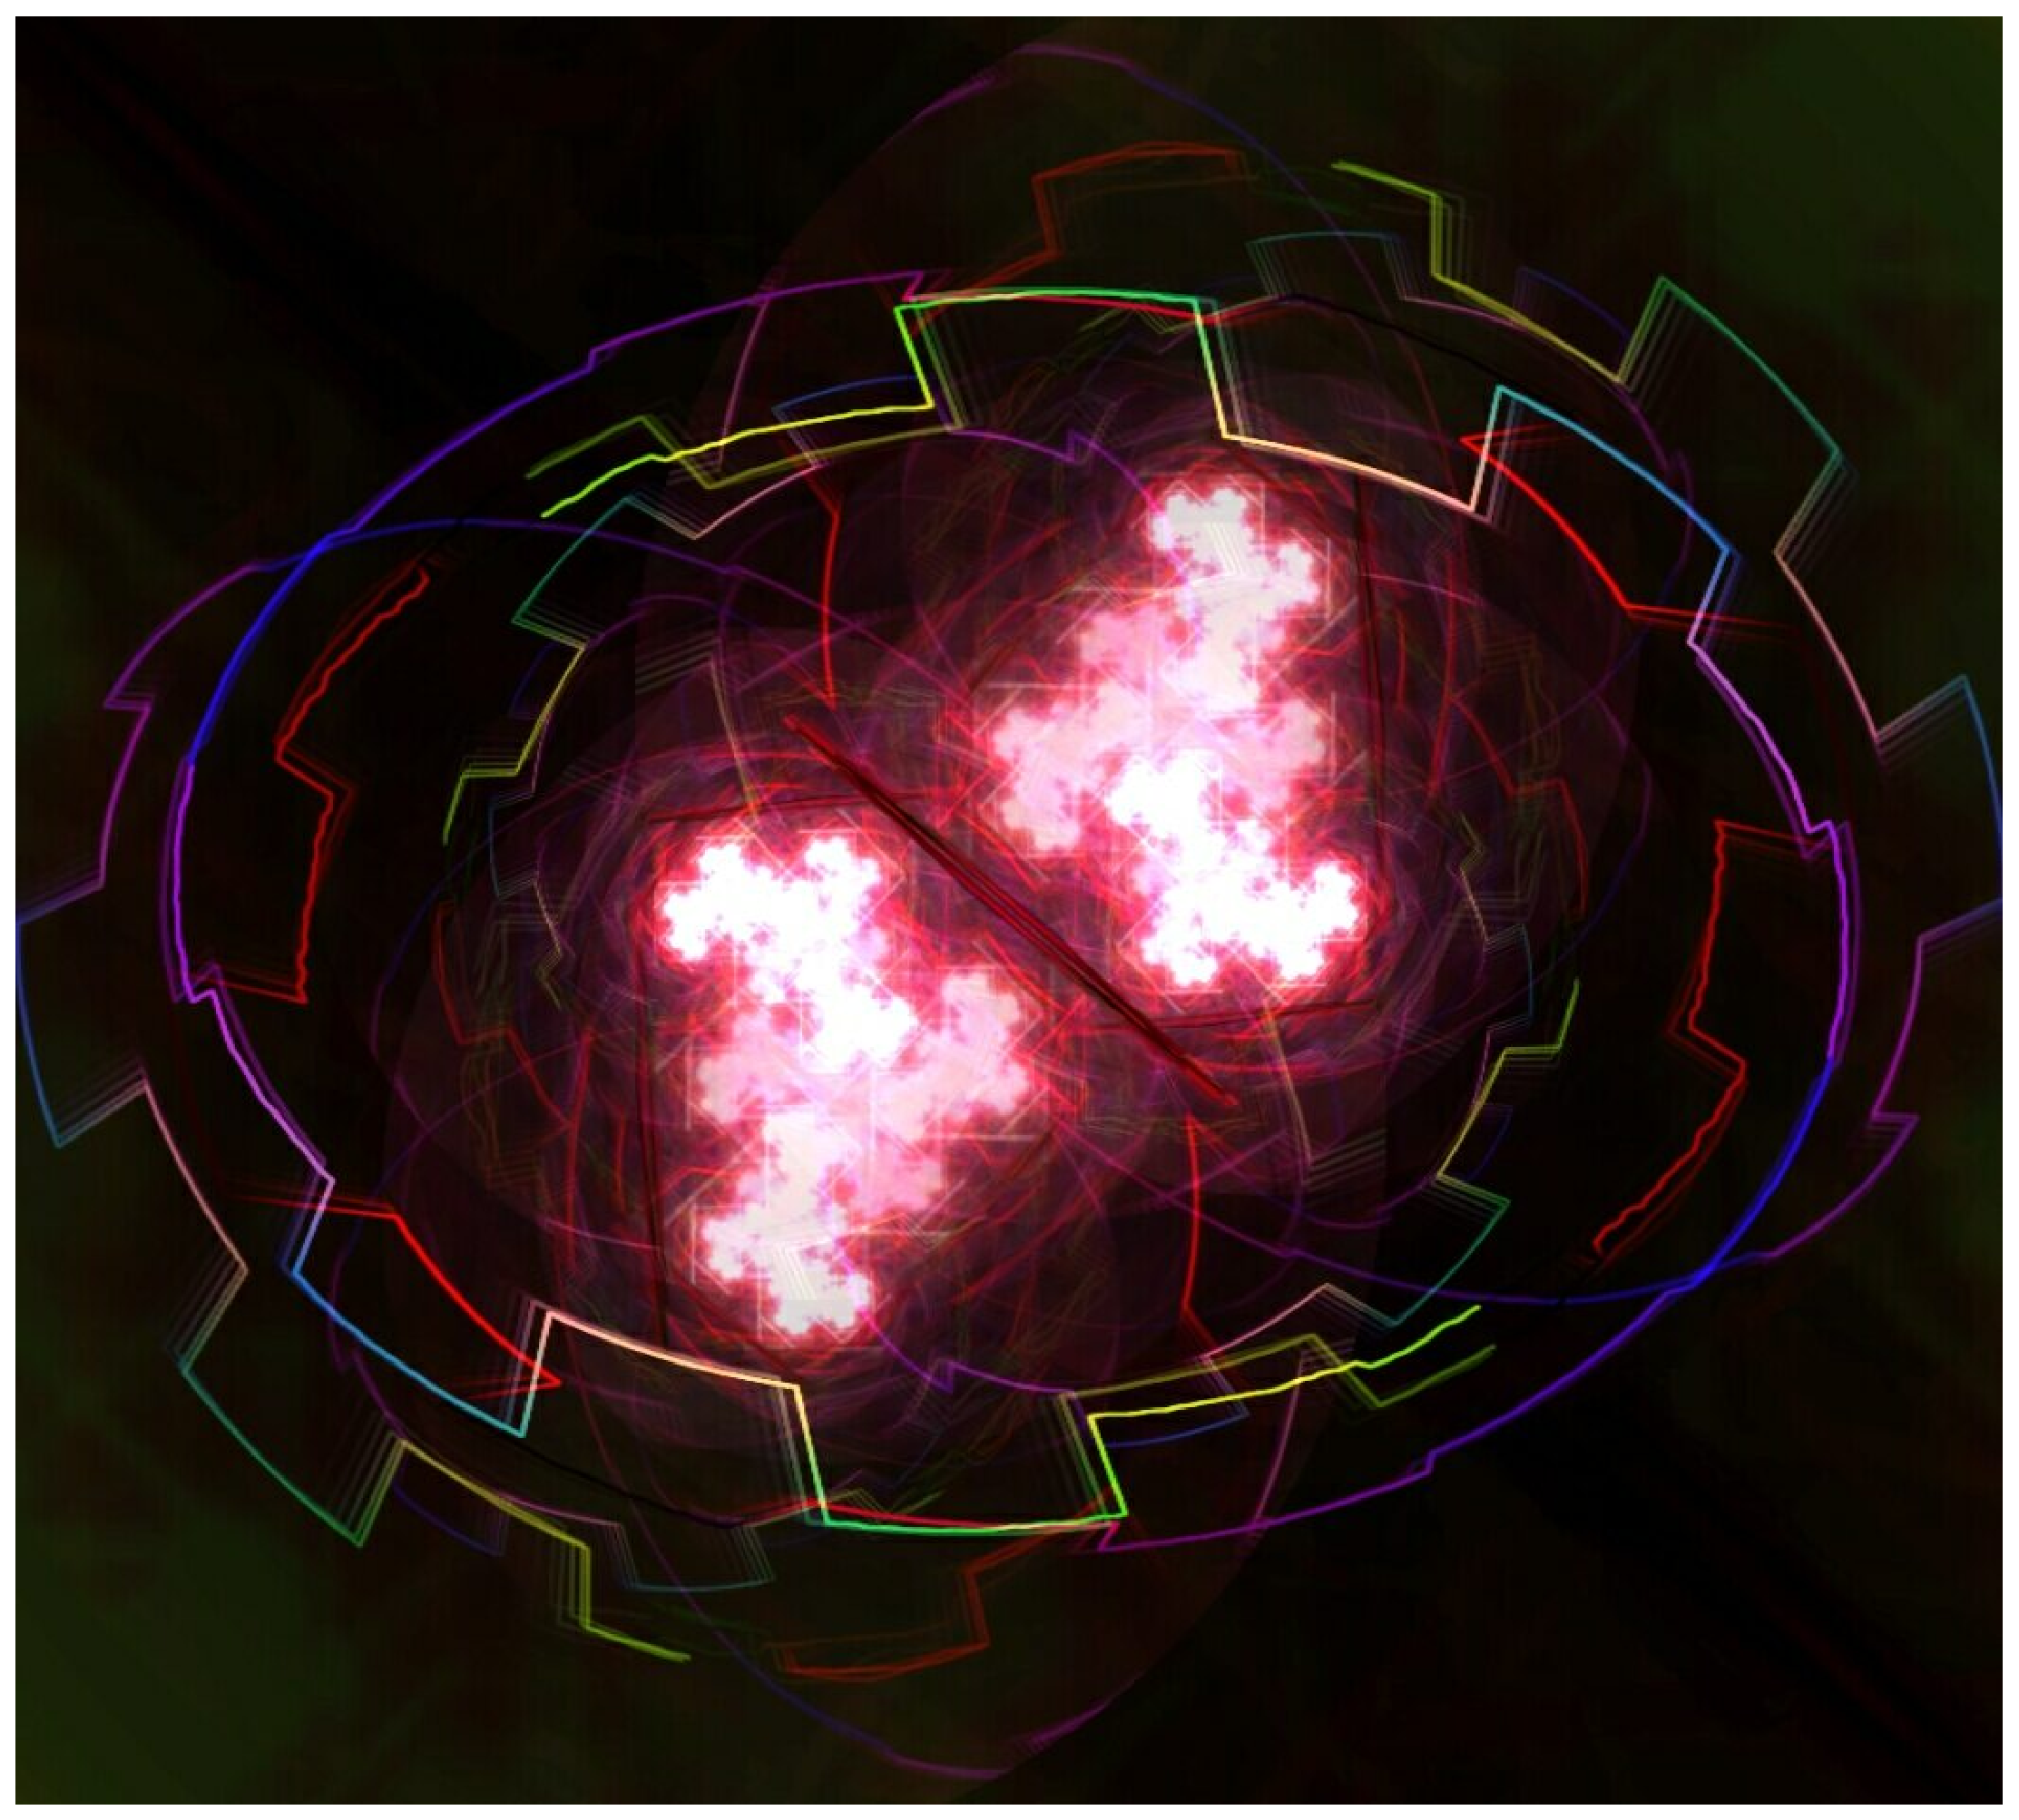
\includegraphics[height=65mm]{milkdrop2.eps}
\caption{Sample video frame from the MilkDrop visual synthesizer.}
\label{fig:milkdrop}
\end{figure}

\subsection{Open source SoC platforms}
There is an existing effort to build open source system-on-chips. It is interesting to review these projects in order to look forward to building upon them -- possibly adding hardware accelerators or performing other modifications in order to improve performance.

There are many SoC designs available on the Internet, which are more or less mature. The system-on-chip projects listed here meet the following criteria:
\begin{itemize}
\item they have been shown to work on at least one FPGA board
\item they are released under an open source license
\item they comprise a synthesizable RISC CPU
\item the CPU is supported by a C and C++ compiler
\item they include a RS232 compatible UART (for a debug console)
\item they support interfacing to off-chip SDRAM memory
\end{itemize}

\subsubsection{OpenSPARC}
OpenSPARC~\cite{opensparc} is the well-known SPARC processor of Sun Microsystems which is now released under an open source license and included into a SoC FPGA project.

Implemented on a FPGA, this processor is extremely resource-intensive. A cut-down version of the CPU core only, called the ``Simply RISC S1'', occupies at least 37000 FPGA look-up tables (LUT) without the caches~\cite{simplyrisc}. This is about twice the logic capacity of the Virtex-4 XC4VLX25 FPGA.

As it turns out, the OpenSPARC architecture is a very complex design which implements a huge number of techniques which increase the software execution speed (instructions per clock cycle). While this is a wise choice for a software-centric processor implemented on a fully custom semiconductor chip, with a FPGA process it is more appealing to keep the software processor simple in order to save resources and make room for custom hardware accelerators, taking advantage of the FPGA flexibility.

\subsubsection{GRLIB}
GRLIB~\cite{grlib} is a very professional and standard-compliant library of SoC cores. The library features a comprehensive set of cores: AMBA AHB/APB bus control elements, the LEON3 SPARC processor, a 32-bit PC133 SDRAM controller, a 32-bit PCI bridge with DMA, a 10/100/1000 Mbit Ethernet MAC,  16/32/64-bit DDR SDRAM/DDR2 SDRAM controllers and more.

However, its drawbacks are:
\begin{itemize}
\item Code complexity. GRLIB is written in VHDL and makes intensive use of custom types, packages, generate statements, etc.
\item Cores are not self-contained. GRLIB defines many ``building blocks'' that are used everywhere else in the code, making it difficult to re-use code in another project which is not based on GRLIB.
\item Significant FPGA resource usage. Synthesized with Xilinx ISE 11.3, a system comprising the LEON3 SPARC processor with a 2-way set-associative 16kB cache and no memory management unit (MMU), the DDR SDRAM controller, a RS232 serial port, and a Ethernet 10/100 MAC uses 13264 FPGA look-up tables (LUT). They map to 79\% of the Virtex-4 XC4VLX25 FPGA. This undermines the possibility of adding hardware acceleration cores.
\item Relatively low clock frequency. With the same parameters as above, the maximum clock frequency is 84MHz.
\end{itemize}

Because of these reasons, GRLIB was not retained.

\subsubsection{ORPSoC (OpenRISC)}
ORPSoC is based on the OpenRISC~\cite{openrisc} processor core, which is the flagship product of OpenCores, a community of developers of open source system-on-chips. ORPSoC is essentially maintained by ORSoC AB.

ORPSoC notably features the OpenRISC OR1200 processor core, the Wishbone~\cite{wishbone} bus, comprehensive debugging facilities, a 16550-compatible RS232 UART, a 10/100Mbps Ethernet MAC and a SDRAM controller.

Unfortunately, ORPSoC is resource-inefficient and extremely slow, mainly because of the OpenRISC implementation which is not optimized for synthesis and the poorly designed SDRAM controller. Using ORSoC AB's reference design, a C program takes more than a dozen of seconds to copy a 16MB SDRAM buffer from one memory location to another.

OpenRISC and ORPSoC therefore do not seem to be a good platform for the performance-demanding video synthesis application.

\subsubsection{LatticeMico32 System}
This product~\cite{mico32} from the FPGA vendor Lattice Semiconductor is comparable to Microblaze~\cite{microblaze} and Nios II~\cite{nios} from its competitors, respectively Xilinx and Altera.

Like its competing products, LatticeMico32 System features a broad library of light, fast and FPGA-optimized SoC cores.

One interesting move made by Lattice Semiconductor is that parts of the LatticeMico32 System are released under an open source license, and most notably the custom LatticeMico32 microprocessor core. LatticeMico32 System is also based upon the Wishbone~\cite{wishbone} bus, whose specification is free of charge and freely distributable.

While it is perhaps technically possible to build Milkymist on top of the LatticeMico32 System, there are licensing issues concerning most notably the DDR SDRAM controller which is proprietary.

However, the LatticeMico32 microprocessor core is interesting. Synthesized for the XC4VLX25 with the 2-way set-associative caches enabled, it occupies only about 2400 LUTs and runs at more than 100MHz.

\section{Problem statement}
According to this background, for the video synthesis application it seems relevant to:

\begin{itemize}
\item develop a fast, resource-efficient and FPGA-optimized system-on-chip
\item develop an efficient memory subsystem
\item use a light-weight softcore CPU
\item develop custom hardware accelerators
\end{itemize}

This thesis focuses on the computer architecture problems and concepts behind these points.

\chapter{Memory subsystem}
\section{Attacking the memory wall}
A recurrent point in many modern computer systems is the memory performance problem. The term \textit{memory wall} was coined~\cite{memorywall} to refer to the growing disparity of performance between logic such as CPUs and off-chip memories. While microprocessor performance has been improving at a rate of 60 percent per year, the access time to DRAM has been improving at less than 10 percent per year~\cite{memvscpu}.

Memory performance is measured with two metrics:
\begin{itemize}
\item \textit{bandwidth}, which is the amount of data that the memory system can transfer during a given period of time.
\item \textit{latency}, which is the amount of time that the memory system spends between the issue of a memory read or write request and its completion.
\end{itemize}

A memory system can have both high bandwidth and latency. If the logic making the memory accesses is able to issue requests in a pipelined fashion, sending a new request without waiting for the previous one to complete, high latency will not have an impact on bandwidth.

Latency and bandwidth are however linked in practice. Decreasing the latency also increases the bandwidth in many cases, because latency blocks sequential processes and prevents them from utilizing the full available bandwidth.

High-end processors for servers and workstations have a good ability to cope with relatively high memory latency, because techniques such as out-of-order execution and hardware multi-threading enable the processor to issue new instructions even though one is blocking on a memory access.

Thus, most of today's SDRAM controllers do a lot to optimize bandwidth but have little focus on latency. Bandwidth-optimizing techniques include:
\begin{itemize}
\item reordering memory transactions to maximize the page mode hit rate.
\item grouping reads and writes together to reduce write recovery times. Along with the above technique, this has a detrimental impact on latency because of the delays incurred by the additional logic in the address datapath.
\item running the system and the SDRAM in asynchronous clock domains in order to be able to run the SDRAM at its maximum allowable clock frequency. This requires the use of synchronizers or FIFOs, which have a high latency.
\item configuring the SDRAM at high CAS latencies in order to increase its maximum allowable clock frequency. This trend is best illustrated by the advent of DDR2 and DDR3 memories whose key innovation is to run their internal DRAM core at a submultiple of the I/O frequency with a wide data bus which is then serialized on the I/O pins. Since the internal DRAM core has a latency comparable to that of the earlier SDR and DDR technologies, the number of CAS latency cycles relative to the I/O clock is also multiplied.
\end{itemize}

An extreme example of these memory controller bandwidth optimizations is the MemMax\textregistered ~DRAM scheduler~\cite{memmax}. This unit sits on top of an already existing memory controller (which already has its own latency), adding seven stages of complex and high-latency pipelining that produces an efficient - but compute-intensive - DRAM schedule. The actual efficiency of this system has been questioned~\cite{dramqos} because of that significant increase in latency.

\section{An alternative approach}
The out-of-order execution and hardware multithreading processor optimizations discussed above are however complex and impractical in the context of small and cheap embedded systems, especially those targetted at small FPGAs. For example, the OpenSPARC~\cite{opensparc}.

\section{Benchmarking}

\chapter{Configuration and Status Register (CSR) bus}
\section{General SoC interconnect: the Wishbone bus and its limitations}
\section{Saving resources and helping timing closure}

\chapter{Software execution environment}
\section{Capabilities}
Linux has been ported to the Milkymist SoC (Figure~\ref{fig:linux}). Since this is a community effort, the details are not covered in this master thesis. Still, this demonstrates the ability of the platform to run complex software.

\begin{figure}[htp]
\centering
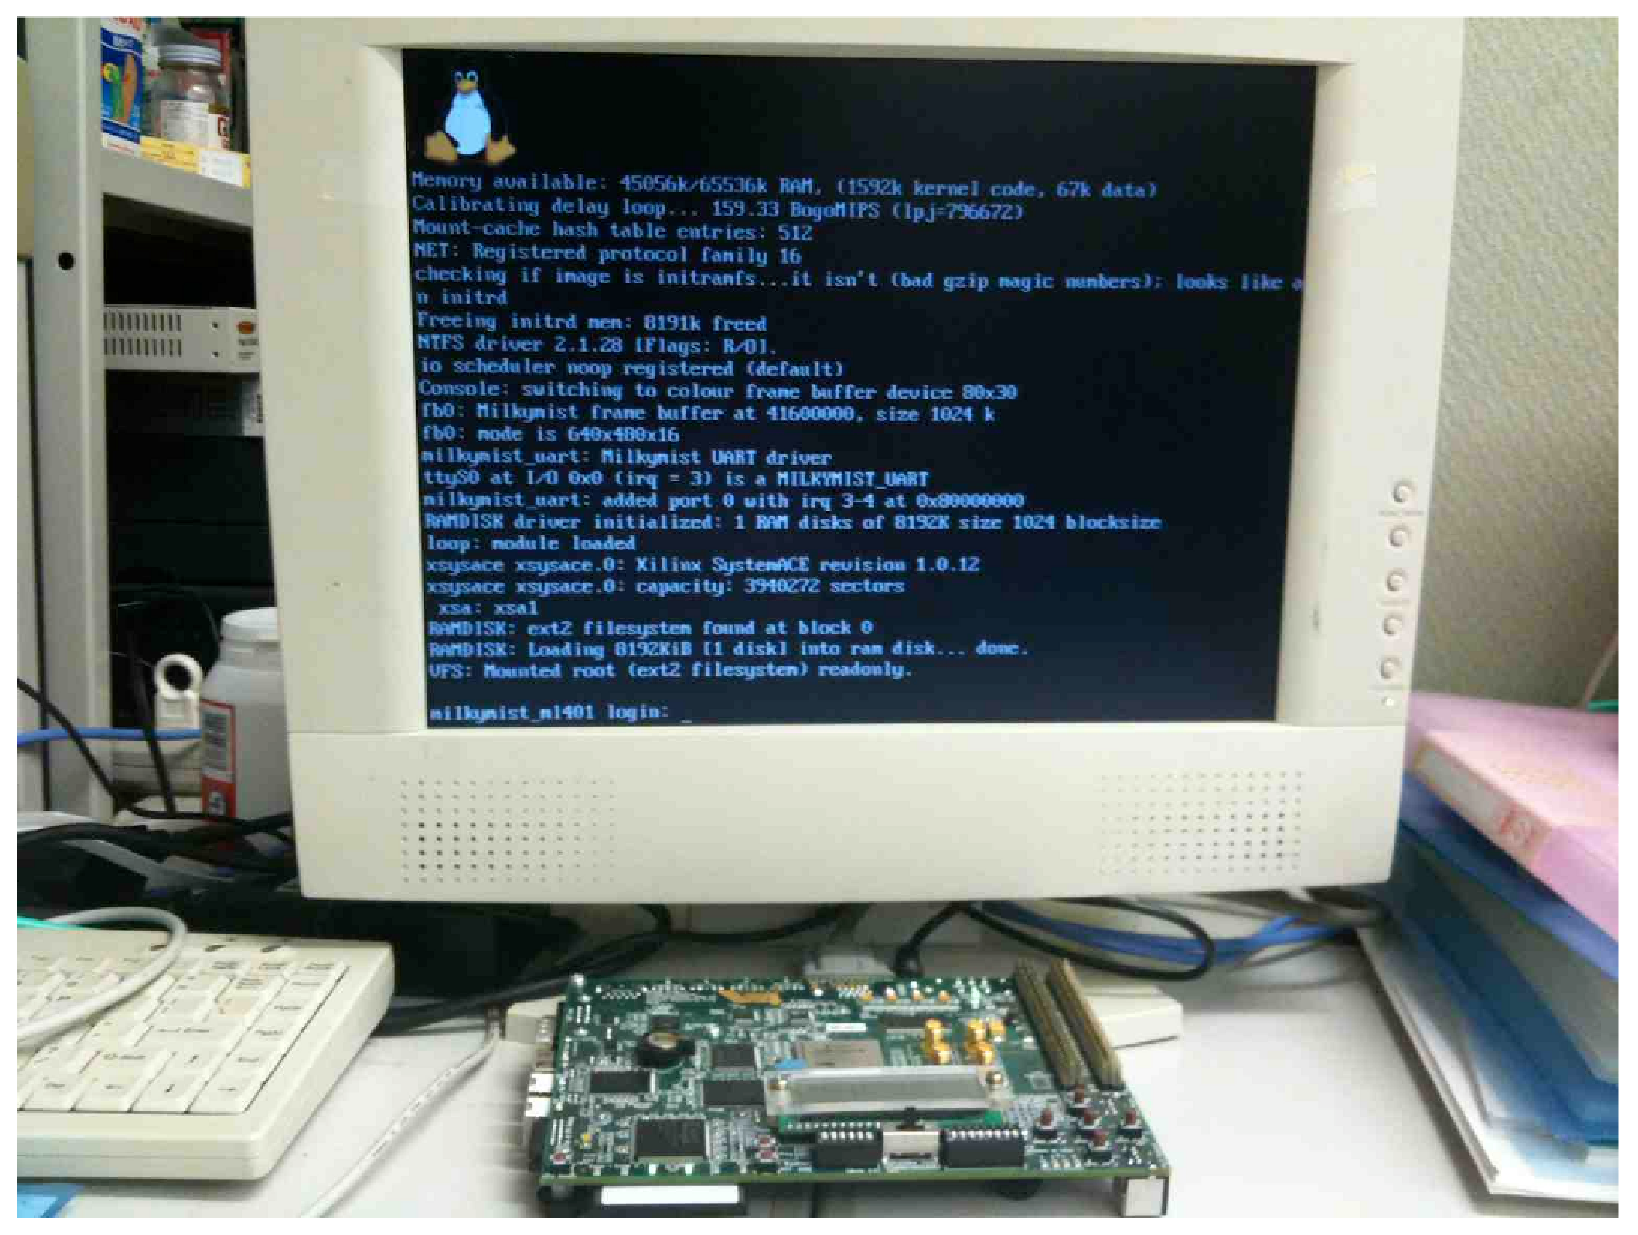
\includegraphics[height=100mm]{linux.eps}
\caption{Linux booting on the Milkymist SoC.}
\label{fig:linux}
\end{figure}

\section{Benchmarking and tuning}

\chapter{Fast texture mapping}

\chapter{The floating point coprocessor}

\bibliography{thesis}{}
\bibliographystyle{plain}

\end{document}
